%%
% La siguiente plantilla esta basada en el siguiente enlace:
% http://academic.reed.edu/physics/courses/Physics332.s08/reports.html
% La plantilla original puede descargarse de ese sitio
% Se dejo parte del texto original en inglés para ilustar el uso de la plantilla
% Se hicieron algunas modificaciones para ajustar el idioma y otros detalles para 
% completar un reporte técnico breve pero muy puntual
% Modificación Inicial: Marco Aurelio Nuno Maganda - 11/SEP/2014
% 
% Enlace a la documentación del tipo de documento base (revtex4)
% http://mirror.hmc.edu/ctan/macros/latex/contrib/revtex/doc/latex/revtex/source/revtex4-1.pdf
%
% En algunas distribuciones es necesario instalar el paquete texlive-publishers
%
%\documentclass[letterpaper,aps,twocolumn,pre,nofootinbib]{revtex4}
%\documentclass[twocolumn]{article}
\documentclass[conference]{IEEEtran}

\usepackage[spanish]{babel}
\usepackage{amsmath,amssymb,amsfonts,amsthm}
\usepackage{graphicx}
%\usepackage{bbm}
\usepackage[utf8]{inputenc} % Caracteres en Español (Acentos, ñs)
\usepackage{url} % ACENTOS
\usepackage{hyperref} % Referencias
\usepackage{subfig}
\usepackage{lipsum}
\usepackage{balance}


%%%%%%%%%%%%%%%%%%%%%%%%%%%%%%%%%%%%%%%%%%%%%
% PARCHE PARA ELIMINAR LA FECHA DEL DOCUMENTO
% 
\usepackage{etoolbox}
\makeatletter
% \frontmatter@RRAP@format is responsible for the parentheses
\patchcmd{\frontmatter@RRAP@format}{(}{}{}{}
\patchcmd{\frontmatter@RRAP@format}{)}{}{}{}
%\renewcommand\Dated@name{}
\makeatother	
% FIN DEL PARCHE
% 
%%%%%%%%%%%%%%%%%%%%%%%%%%%%%%%%%%%%%%%%%%%%%

%%%%%%%%%%%%%%%%%%%%%%%%%%%%%%%%%%%%%%%%%%%%%
% PARCHE PARA PERMIRIR UTILIZAR BIBLATEX EN ESTA PANTLLA
%\PassOptionsToPackage{square,numbers}{natbib}
%\RequirePackage{natbib}  
%%%%%%%%%%%%%%%%%%%%%%%%%%%%%%%%%%%%%%%%%%%%%

\usepackage[backend=bibtex,sorting=none]{biblatex}
% Estas lineas permiten romper los hipervinculos muy largos !!!!
\setcounter{biburllcpenalty}{7000}
\setcounter{biburlucpenalty}{8000}
\addbibresource{references.bib}

% Actualiza en automático la fecha de las citas de internet a la fecha de la compilación del documento
\usepackage{datetime}
\newdateformat{specialdate}{\twodigit{\THEDAY}-\twodigit{\THEMONTH}-\THEYEAR}
\date{\specialdate\today}

% la sentencia \burl en las citas... 
\usepackage[hyphenbreaks]{breakurl}

\renewcommand\spanishtablename{Tabla}
\renewcommand\spanishfigurename{Figura}

%\usepackage{datetime}
%\newdateformat{specialdate}{\twodigit{\THEDAY}-\twodigit{\THEMONTH}-\THEYEAR}
%\newdateformat{specialdate}{\twodigit{\THEDAY}-\THEYEAR}
%\date{\specialdate\today}


\begin{document}
%%%%%%%%%%%%%%%%%%%%%%%%%%%%%%%%%%%%%%%%%%%%%
% Definitions
%
%
% Define your special symbols here
%
%%%%%%%%%%%%%%%%%%%%%%%%%%%%%%%%%%%%%%%%%%%%%

% use to set width of figures
\newcommand{\breite}{0.9} %  for twocolumn
\newcommand{\RelacionFiguradoscolumnas}{0.9}
\newcommand{\RelacionFiguradoscolumnasPuntoCinco}{0.45}


%%%%%%%%%%%%%%%%%%%%%%%%%%%%%%%%%%%%%%%%%%%%%
% End Definitions
%%%%%%%%%%%%%%%%%%%%%%%%%%%%%%%%%%%%%%%%%%%%%


%Title of paper
\title{Convertidor de Volúmen con Pyhton y PyQt6}

% Trabajo Individual
\author{\IEEEauthorblockN{ALAN EMANUEL MORALES SALAZAR\IEEEauthorrefmark{1}}
% En caso de trabajos en equipo, poner a todos los autores en estricto ORDEN ALFABETICO
%\author{\IEEEauthorblockN{Michael Shell\IEEEauthorrefmark{1},
%Homer Simpson\IEEEauthorrefmark{1},
%James Kirk\IEEEauthorrefmark{1}, 
%Montgomery Scott\IEEEauthorrefmark{1} and
%Eldon Tyrell\IEEEauthorrefmark{1}}
\IEEEauthorblockA{\IEEEauthorrefmark{1}Ingeniería en Tecnologías de la Información\\
Universidad Politécnica de Victoria}
}


%\date{}

\maketitle

\begin{abstract} 
Este documento describe una aplicación desarrollada en Python usando la librería de PyQt6 para la GUI, esta aplicación está diseñada para calcular el volumen de un cubo. La aplicación permite al usuario elegir entre el tipo de unidad que puede ingresar para calcular el volumen, además que puede elegir la unidad de medida que quiere que muestre el volumen. 
\end{abstract}


%\maketitle must follow title, authors, abstract, \pacs, and \keywords




\section{Introducción}

El cálculo de volúmenes es una tarea fundamental en diversas áreas, desde la educación hasta la ingeniería. Con el objetivo de facilitar este proceso, se desarrolló una aplicación en Python \cite{python} utilizando PyQt6 \cite{pyqt6} para crear una interfaz gráfica amigable para todas las personas. Esta herramienta permite a los usuarios ingresar las dimensiones de un cubo en centímetros o pulgadas y obtener su volumen en distintas unidades de medida. Además, la aplicación incorpora elementos interactivos como botones y spinBox para mejorar la experiencia del usuario.
 
\section{Desarrollo Experimental}

En este trabajo se desarrolló una aplicación para calcular el volumen de un cubo \cite{Omni2025}. Para esto se tomó de referencia el convertidor de volumen que se encuentra en la página de online-calculator \cite{volumeConverter}. El desarrollo de esta aplicación se elaboró utilizando Python \cite{qtforpython} y la librería PyQt6 de la bibiloteca de Qt. En esta aplicación el usuario puede ingresar los valores de largo, ancho y alto que el desee, el usuario también tiene la opción si quiere ingresar los valores en centímetros (cm) o en pulgadas (inch), además que puede elegir la unidad de medida que quiere que se muestre el resultado del volumen, las opciones son metros cúbicos (m³), pies cúbicos (ft³) y centímetros cúbicos (cm³). En esta ocasión la librería de PyQt6 \cite{DELAOSSAALIAN2025101497} ayudó en la creación de GUI \cite{5725235}. Primero se hizo la cosa más importante, lo cual es el desarrollo de la GUI, primero se comenzó con la distribución de los layouts, la aplicación contiene un layout main el cual es horizontal, y dentro de ella tiene dos layouts más, pero estos son verticales.

En la parte superior de la GUI se implementaron dos botones principales, los cuales son los de CM y Inch. Para hacer la calculadora muy similar al convertidos que está en la página de referencia, tenía que implementar spinBox \cite{qspinbox} en lugar de inputs comúnes. Y para que el label y el spinBox estuvieran al mismo nivel tuve que agregar dentro del layout izquierdo 4 layouts horizontales, 3 de esos layouts son para el label y el spinBox y uno de ellos es para los botones de unidades que el usuario podría elegir.

Para el layout derecho simplemente se agregaron dos labels y la misma imagen del cubo que tenía la página de referencia. Esta GUI se puede ver en la Figura\ref{fig:figura1}.

%%%%%%%%%%%%%%%%%%%%%%%%%%%%%%%%%%%%%%%%%%%%%%%%%%%%
% FIGURE 1
%%%%%%%%%%%%%%%%%%%%%%%%%%%%%%%%%%%%%%%%%%%%%%%%%%%%
%
%
% 
\begin{figure}
{\includegraphics*[width=\breite\columnwidth]{GUI.png}}
%\includegraphics*[width=\breite \columnwidth]{Fig1} 
\caption{Interfaz gráfica del usuario (GUI)}
\label{fig:figura1}
\end{figure}

%%%%%%%%%%%%%%%%%%%%%%%%%%%%%%%%%%%%%%%%%%%%%%%%%%%%

Para la creación de los layouts que almacenan lo mismo, se hizo una función en la que solo se le mandan el label y el spinBox y está función solo regresa el layout ya con el label y el spinBox acomodados, lo mismo se hizo para los botones que cambian la unidad en la que quieren que se muestre el volumen.
Para que el resultado del calculo del volumen se actualice al instante en que el usuario modifica los valores se tuvo que mandar los valores que ingresaba el usuario directamente a la función que calcula el volumen.

En la creación de los spinBox obligatoriamente le tuve que dar valores máximos y mínimos, en este caso puse 0 como valor mínimo, y puse 1 trillón como valor máximo, aunque debo que admitir que el único problema que tuve fue que al ser el numero tan largo este no se muestra completo ya que se sale de los limites.

El código fue ejecutado en una computadora con un procesador AMD Ryzen 5 5600H y 16 GB de memoria RAM. La ejecución de la aplicación fue óptima para este equipo, por lo que se espera lo mismo para equipos que cuenten con características similares.
%%%%%%%%%%%%%%%%%%%%%%%%%%%%%%%%%%%%%%%%%%%%%%%%%%%%


\section{Resultados}

A continuación, se demuestra la ejecución del código. Primeramente como se dijo anteriormente se muestra la interfaz principal [\ref{fig:figura1}], en ella se muestran todas las características que se mencionaron dentro del desarrollo, los cuales son los botones, los label y los spinBox. En la Figura \ref{fig:figure2} se presentan diferentes pantallas de la interfaz. Como se mencionó anteriormente, en la parte superior hay dos botones, en los que el usuario puede elegir entre centímetros, como se muestra en la Figura \ref{fig:figure2}(a), y pulgadas como se muestra en la Figura \ref{fig:figure2}(b). 
Por otro lado, en la Figura \ref{fig:figure3}, también se muestran diferentes pantallas de la interfaz. Además de los botones que se encuentran en la parte superior también hay botones en la parte inferior, solo que estos son redondos, el usuario al darle clic a algunos de estos la unidad de medida del resultado del volumen va a cambiar.

%%%%%%%%%%%%%%%%%%%%%%%%%%%%%%%%%%%%%%%%%%%%%%%%%%%%
% FIGURE 2
%%%%%%%%%%%%%%%%%%%%%%%%%%%%%%%%%%%%%%%%%%%%%%%%%%%%

\begin{figure}
%\includegraphics*[width= \breite \columnwidth]{Fig2} 
%\includegraphics*[width= 1.6 \columnwidth]{Fig2} 
\subfloat[Medidas del cubo en caso de calcular el volumen en centímetros]{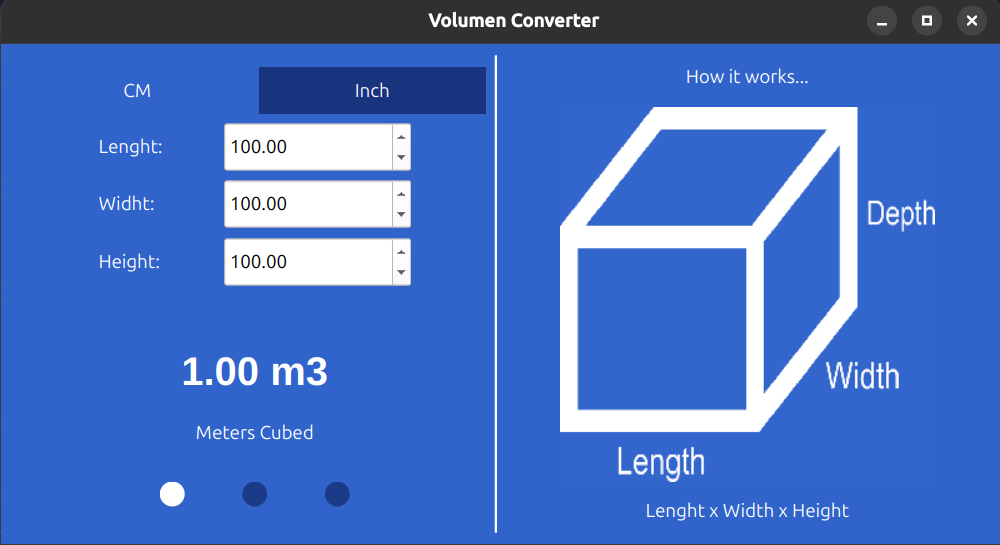
\includegraphics[width= \breite \linewidth]{GUI.png}}\\
\subfloat[Medidas del cubo en caso de calcular el volumen en pulgadas]{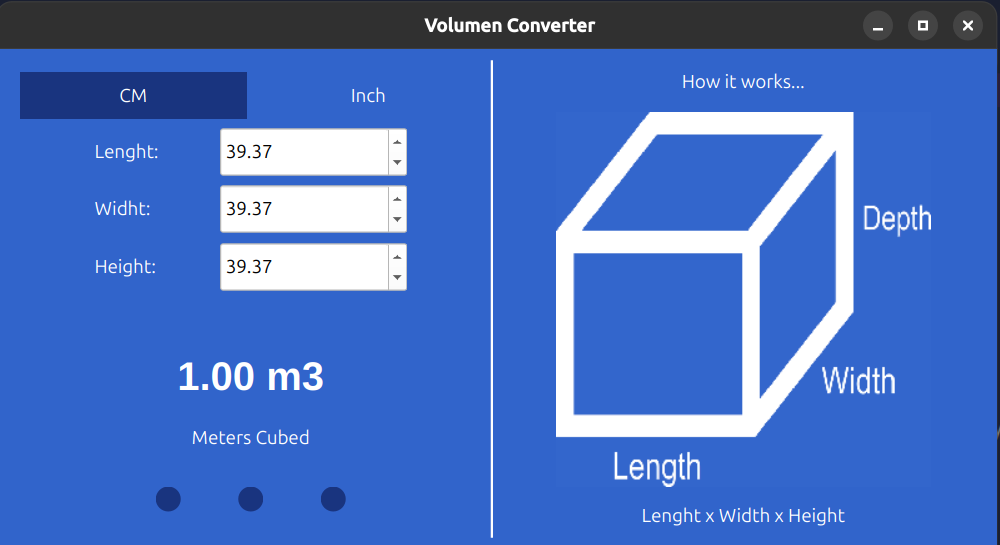
\includegraphics[width= \breite \linewidth]{valores-en-pulgadas.png}}\\
\caption{Medidas del cubo. (a). En centímetros. (b). En pulgadas. 
}
\label{fig:figure2}
\end{figure}

%%%%%%%%%%%%%%%%%%%%%%%%%%%%%%%%%%%%%%%%%%%%%%%%%%%%
% FIGURE 3
%%%%%%%%%%%%%%%%%%%%%%%%%%%%%%%%%%%%%%%%%%%%%%%%%%%%
%
%
% 
\begin{figure}
%\begin{subfigure}[b]{\textwidth}
            %    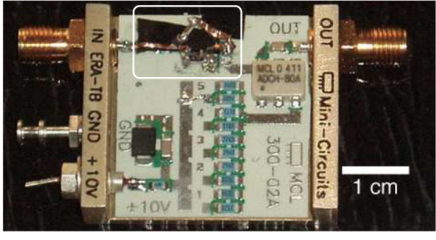
\includegraphics[width=\breite \columnwidth]{Fig1a}
         %       \caption{A gull}
   %             \label{fig:gull}
      %  \end{subfigure}
\subfloat[Resultado en metros cúbicos (m³)]{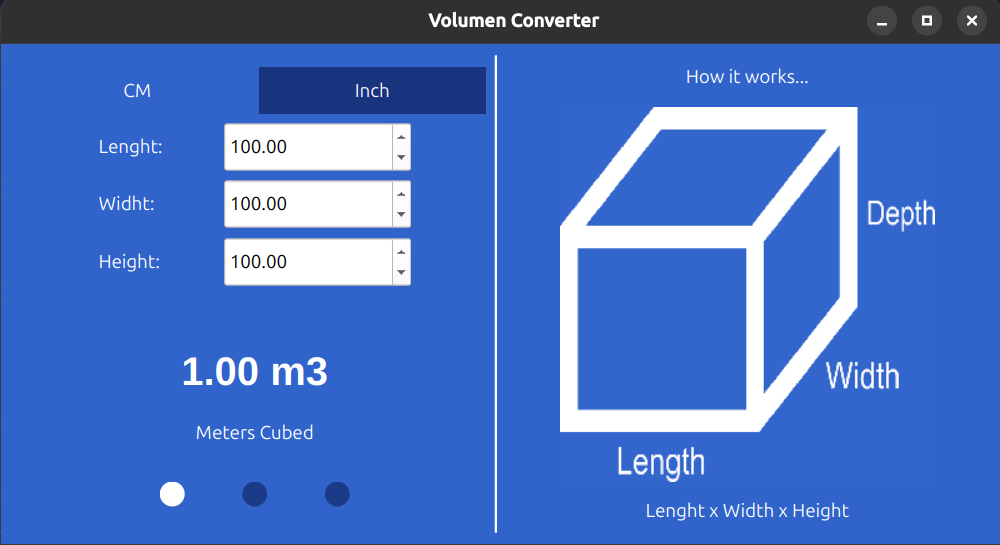
\includegraphics[width=\breite\linewidth]{GUI.png}}\\
\subfloat[Resultado en pies cúbicos (ft³)]{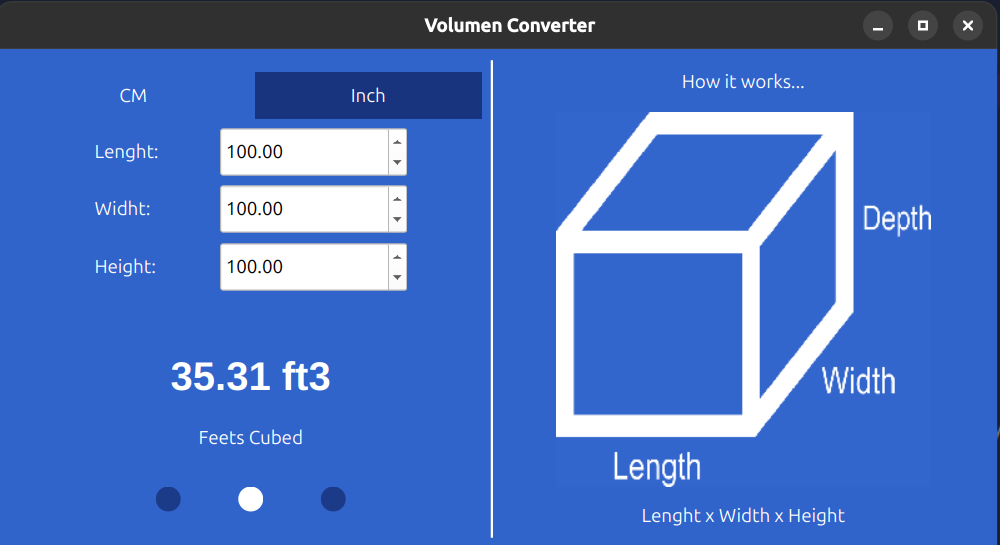
\includegraphics[width=\breite\linewidth]{resultado-pies.png}}\\
\subfloat[Resultado en centímetros cúbicos (cm³)]{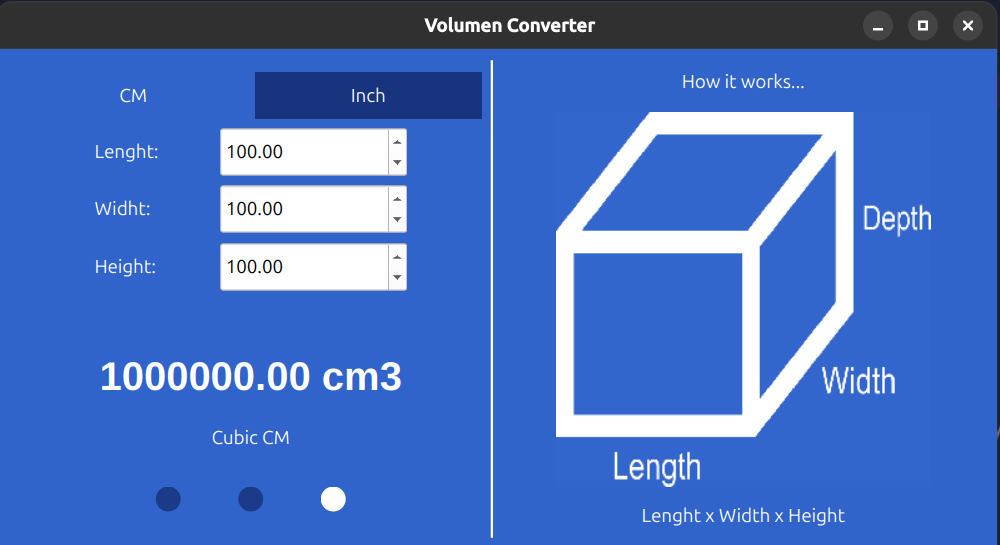
\includegraphics[width=\breite\linewidth]{resultado-centimetros.png}}
\caption{Resultado del volumen en distintas unidades: a) Metros Cúbicos; b) Pies Cúbicos; c) Centímetros Cúbicos
}
\label{fig:figure3}
\end{figure}


\section{Conclusión}

En este documento se ha presentado una aplicación que ayuda al cálculo de volumen de un cubo, esta aplicación fue desarrollada en Python \cite{gonzalez2023} y con la librería de PyQt6. Esta aplicacion permite a los usuarios ingresar valores en distintas unidades y obtener el resultado de forma dinámica \cite{cuevas2023}.

Durante el proceso de desarrollo, se enfrentaron desafíos como la organización de los layouts y la actualización en tiempo real de los cálculos, los cuales fueron resueltos con una adecuada implementación de los elementos de la GUI. 

En general, la aplicación cumple con su propósito de calcular el volumen de un cubo de manera eficiente, ofreciendo al usuario una herramienta práctica y fácil de usar.


\addcontentsline{toc}{section}{Referencias} 
\printbibliography
%\balance



\end{document}













